\section{Database entities \& relationships}

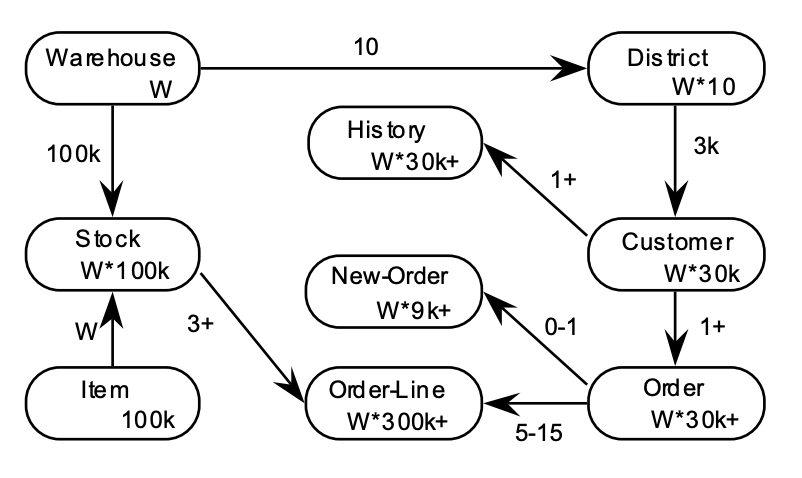
\includegraphics{img/relationships.png}

- The numbers in the entity blocks represent the cardinality of the tables (number of rows). These numbers are factored by W, the number of Warehouses, to illustrate the database scaling.

- The numbers next to the relationship arrows represent the cardinality of the relationships (average number of children per parent).

- The plus (+) symbol is used after the cardinality of a relationship or table to illustrate that this number is subject to small variations in the initial database population over the measurement interval (see Clause 5.5) as rows are added or deleted.

\section{Table layouts}

\subsection{WAREHOUSE Table Layout}

\begin{center}
\begin{tabular}{ |c|c|m{7.5cm}| } 
 \hline
 Field Name & Field Definition & Comments \\ 
 \hline
 \rowcolor{gray}
 wId & 2*W unique IDs & W Warehouses are populated \\ 
 name & variable text, size 10 &  \\ 
 str1 & variable text, size 20 & Address line 1 \\
 str2 & variable text, size 20 & Address line 2 \\
 city & variable text, size 20 &  \\
 state & fixed text, size 2 & \\
 zip & fixed text, size 9 &  \\
 tax & signed numeric(4,4) & Sales tax \\
 wYTD & signed numeric(12,2) & Year to date balance \\

 \hline
\end{tabular}
\end{center}

\subsection{DISTRICT Table Layout}

\begin{center}
\begin{tabular}{ |c|c|m{7.5cm}| } 
 \hline
 Field Name & Field Definition & Comments \\ 
 \hline
 \rowcolor{gray}
 dId & 20 unique IDs & 10 are populated per warehouse\\
\rowcolor{gray}
 wId* & 2*W unique IDs & Associated warehouse \\ 
 name & variable text, size 10 &  \\ 
 str1 & variable text, size 20 & Address line 1 \\
 str2 & variable text, size 20 & Address line 2 \\
 city & variable text, size 20 &  \\
 state & fixed text, size 2 & \\
 zip & fixed text, size 9 &  \\
 tax & signed numeric(4,4) & Sales tax \\
 dYTD & signed numeric(12,2) & Year to date balance \\
 nextOrdId & 10,000,000 unique IDs & Next available Order number, increment by 1 every time new order is added \\
 \hline
\end{tabular}
\end{center}

\subsection{CUSTOMER Table Layout}

\begin{center}
\begin{tabular}{ |c|c|m{7.5cm}| } 
 \hline
 Field Name & Field Definition & Comments \\ 
 \hline
 \rowcolor{gray}
 cId & 96,000 unique IDs & 3,000 are populated per district\\
 \rowcolor{gray}
 dId & 20 unique IDs & Associated warehouse\\
 \rowcolor{gray}
 wId & 2*W unique IDs & Customer-warehouse ID \\ 
 first & variable text, size 16 & First name\\
 middle & fixed text, size 2 & Middle initials (max 2)\\
 last & variable text, size 16 & Last name \\ 
 str1 & variable text, size 20 & Address line 1 \\
 str2 & variable text, size 20 & Address line 2 \\
 city & variable text, size 20 &  \\
 state & fixed text, size 2 & \\
 zip & fixed text, size 9 &  \\
 phone & fixed text, size 16 & \\
 since & date and time & \\
 credit & fixed text, size 2 & "GC"=good, "BC"=bad\\
 credLim & signed numeric(12, 2) & \\
 discount & signed numeric(4, 4) & \\
 balance & signed numeric(12, 2) & \\
 YTDPaymt & signed numeric(12, 2) & Customer payment year to date\\
 paymtCnt & numeric(4) & Customer payment count \\
 deliveryCnt & numeric(4) & \\
 data & variable text, size 500 & Miscellaneous information \\
 \hline
\end{tabular}
\end{center}

\subsection{HISTORY Table Layout}

\begin{center}
\begin{tabular}{ |c|c|m{7.5cm}| } 
 \hline
 Field Name & Field Definition & Comments \\ 
 \hline
 cId* & 96,000 unique IDs &\\

 cDId* & 20 unique IDs &\\

 cWId* & 2*W unique IDs & \\ 
 dId* & 20 unique IDs & \\
 wId* & 2*W unique IDs & \\ 
 date & date and time & \\
 amount & signed numeric(6, 2) & \\
 data & variable text, size 24 & Miscellaneous information \\
 \hline
\end{tabular}
\end{center}
Comment: Rows in the History table do not have a primary key as, within the context of the benchmark, there is no need to uniquely identify a row within this table. 

\subsection{NEW-ORDER Table Layout}

\begin{center}
\begin{tabular}{ |c|c|m{7.5cm}| } 
 \hline
 Field Name & Field Definition & Comments \\ 
 \hline
 \rowcolor{gray}
 oId & 10,000,000 unique IDs & \\
 dId* & 20 unique IDs &\\
 wId* & 2*W unique IDs & \\ 
 \hline
\end{tabular}
\end{center}

\subsection{ORDER Table Layout}

\begin{center}
\begin{tabular}{ |c|c|m{7.5cm}| } 
 \hline
 Field Name & Field Definition & Comments \\ 
 \hline
 \rowcolor{gray}
 oId & 10,000,000 unique IDs & \\
 \rowcolor{gray}
 dId* & 20 unique IDs & \\
 \rowcolor{gray}
 wId* & 2*W unique IDs & \\ 
 cId* & 96,000 unique IDs & \\
 entryDate & date and time & \\
 carrierId & 10 unique IDs, or null & \\
 oLCnt & numeric(2) & Count of Order-Lines (number of items) \\
 allLocal & numeric(1) & If all local then 1 else 0\\
 \hline
\end{tabular}
\end{center}

\subsection{ORDER-LINE Table Layout}

\begin{center}
\begin{tabular}{ |c|c|m{7cm}| } 
 \hline
 Field Name & Field Definition & Comments \\ 
 \hline
 \rowcolor{gray}
 oId* & 10,000,000 unique IDs & \\
 \rowcolor{gray}
 dId* & 20 unique IDs & \\
 \rowcolor{gray}
 wId* & 2*W unique IDs & \\ 
 \rowcolor{gray}
 number & 15 unique IDs & \\
 iId & 200,000 unique IDs & Item ID \\
 supplyWId & 2*W unique IDs  & \\
 deliveryDate & date and time, or null & \\
 quantity & numeric(2)  & \\
 amount & signed numeric(6, 2) & \\ 
 distInfo & fixed text, size 24 & \\
 \hline
\end{tabular}
\end{center}


\subsection{ITEM Table Layout}

\begin{center}
\begin{tabular}{ |c|c|m{7cm}| } 
 \hline
 Field Name & Field Definition & Comments \\ 
 \hline
 \rowcolor{gray}
 iId & 200,000 unique IDs  & 100,000 items are populated \\
 iMId & 200,000 unique IDs & Image ID associated to Item \\
 name & variable text, size 24 & \\
 price & numeric(5, 2) & \\
 data & variable text, size 50 & Brand information \\

 \hline
\end{tabular}
\end{center}

\subsection{STOCK Table Layout}

\begin{center}
\begin{tabular}{ |c|c|m{7cm}| } 
 \hline
 Field Name & Field Definition & Comments \\ 
 \hline
 \rowcolor{gray}
 iId & 200,000 unique IDs  & 100,000 items are populated \\
 \rowcolor{gray}
 wId & 2*W unique IDs & \\
 quantity & signed numeric(4) & \\
 dist01 & fixed text, size 24 & \\
 dist02 & fixed text, size 24 & \\
 dist03 & fixed text, size 24 & \\
 dist04 & fixed text, size 24 & \\
 dist05 & fixed text, size 24 & \\
 dist06 & fixed text, size 24 & \\
 dist07 & fixed text, size 24 & \\
 dist08 & fixed text, size 24 & \\
 dist09 & fixed text, size 24 & \\
 dist10 & fixed text, size 24 & \\
 YTD & numeric(8) & \\
 orderCnt & numeric(4) & \\
 remoteCnt & numeric(4) & \\
 data & variable text, size 50 & Information\\
 \hline
\end{tabular}
\end{center}